\documentclass[titlepage = firstcover]{scrartcl}
\usepackage[aux]{rerunfilecheck}
\usepackage{fontspec}
\usepackage[main=ngerman, english, french]{babel}

% mehr Pakete hier
\usepackage{expl3}
\usepackage{xparse}

%Mathematik------------------------------------------------------
\usepackage{amsmath}   % unverzichtbare Mathe-Befehle
\usepackage{amssymb}   % viele Mathe-Symbole
\usepackage{mathtools} % Erweiterungen für amsmath
\usepackage{dsfont}
\usepackage[
  math-style=ISO,    % \
  bold-style=ISO,    % |
  sans-style=italic, % | ISO-Standard folgen
  nabla=upright,     % |
  partial=upright,   % /
]{unicode-math}% "Does exactly what it says on the tin."
\usepackage[section, below]{placeins}

% Laden von OTF-Mathefonts
% Ermöglich Unicode Eingabe von Zeichen: α statt \alpha

\setmathfont{Latin Modern Math}
%\setmathfont{Tex Gyre Pagella Math} % alternativ zu Latin Modern Math
\setmathfont{XITS Math}[range={scr, bfscr}]
\setmathfont{XITS Math}[range={cal, bfcal}, StylisticSet=1]

\AtBeginDocument{ % wird bei \begin{document}
  % werden sonst wieder von unicode-math überschrieben
  \RenewDocumentCommand \Re {} {\operatorname{Re}}
  \RenewDocumentCommand \Im {} {\operatorname{Im}}
}
\usepackage{mleftright}
\setlength{\delimitershortfall}{-1sp}
\usepackage[version=4]{mhchem}

%Sprache----------------------------------------------------------
\usepackage{microtype}
\usepackage{xfrac}
\usepackage[autostyle]{csquotes}    % babel
\usepackage[german, unicode, pdfusetitle]{hyperref}
\usepackage{bookmark}
\usepackage[shortcuts]{extdash}
%Einstellungen hier, z.B. Fonts
\usepackage{booktabs} % Tabellen

\setlength{\parindent}{0pt}

\title{US2 - Scanverfahren in der Ultraschalltechnik}
\author{
  David Gutnikov\\
  \href{mailto:david.gutnikov@udo.edu}{david.gutnikov@udo.edu}\\
  Lasse Sternemann\\
  \href{mailto:lasse.sternemann@udo.edu}{lasse.sternemann@udo.edu}
}
\date{Bearbeitet am 7.07.2020}

\begin{document}
    \maketitle
    \newpage
    \tableofcontents
    \newpage

    \section{Auswertung}
        Aufgrund mangelnder Kompetenz ist dem Programm nicht die Laufzeit des Schalls, sondern direkt die Tiefe der Löcher entnommen worden. Deswegen werden diese Werte direkt mit den mit Hilfe
        einer Schiebelehre gemessenen Werten verglichen und anschließend die theoretische Laufzeit des Schalls bei entsprechender Tiefe berechnet.

        \FloatBarrier

        \begin{figure}[h]
          \centering
          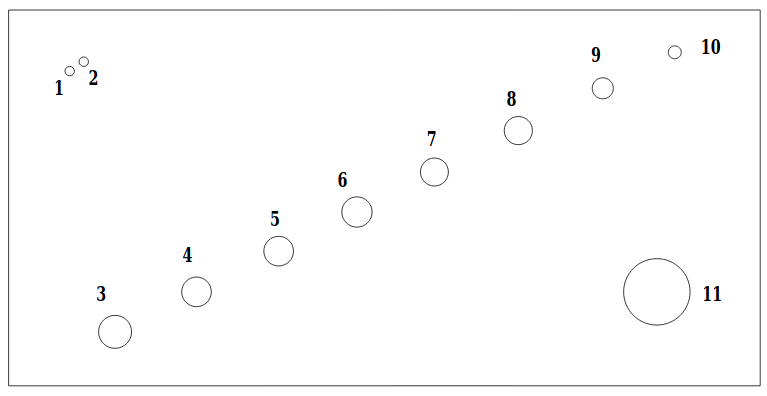
\includegraphics[width = 0.8\textwidth]{Bilder/DerBlock.png}
          \caption{In der Abbildung ist der untersuchte Acrylblock zu sehen.}
          \label{fig:DerBlock}
        \end{figure}

        \FloatBarrier

        \noindent


        \subsection{Amplituden-Scan}
            In der ersten Tabelle \ref{tab:Abstand1} sind die Abstände der Löcher 3, 4, 5, 6 und 7 von der in Skizze \ref{fig:DerBlock} unten liegenden Seite per Messung mit der Schiebelehre und per Messung durch den 
            Ampliuden-Scan eingetragen. Zusätzlich wird die Abweichung des per Amplituden-Scans gemessenen Abstands zum Wert der Schiebelehre, sowie die theoretische Laufzeit der Schallwelle im
            Acrylblock berechnet und in die Tabelle eingetragen. Zur Berechnung der Laufzeit wird Formel x nach t umgestellt.

            \begin{table}[h]
                \centering
                \caption{In der Tabelle sind die gemessenen Abstände, sowie deren Abweichung und die theoretische Laufzeit des Schalls, unter Vorraussetzung der richtig gewählten spezifischen Schallgeschwindigkeit im Programm, eingetragen.}
                \label{tab:Abstand1}

                \begin{tabular}{c c c c c}
                    \toprule
                    {Loch} & {Abstand SL [mm]} & {Abstand A-Scan [mm]} & {Abweichung [\%]} & {Laufzeit [$\mu$s]}  \\
                    \midrule
                    3   &   13,30$\pm$0,02   &   16$\pm$1  &   20,30   &   11.99$\pm$0,75   \\
                    4   &   21,80$\pm$0,02   &   24$\pm$1  &   10,09   &   17,98$\pm$0,75   \\
                    5   &   30,14$\pm$0,02   &   33$\pm$1  &   9,49    &   24,72$\pm$0,75   \\
                    6   &   38,60$\pm$0,02   &   41$\pm$1  &   6,22    &   30,71$\pm$0,75   \\
                    7   &   46,58$\pm$0,02   &   49$\pm$1  &   5,20    &   36,70$\pm$0,75   \\       
                    \bottomrule
                \end{tabular}

            \end{table}

            \FloatBarrier
            \noindent
            In der nun folgenden Tabelle sind die gleichen Messungen sowie Berechnungen für die Abstände der Löcher 3, 4, 5, 6 und 7 von der in der Skizze \ref{fig:DerBlock} links liegenden Seite eingetragen.
            
            \begin{table}[h]
              \centering
              \caption{In der Tabelle sind die gemessenen Abstände, sowie deren Abweichung und die theoretische Laufzeit des Schalls, unter Vorraussetzung der richtig gewählten spezifischen Schallgeschwindigkeit im Programm, eingetragen.}
              \label{tab:Abstand2}

              \begin{tabular}{c c c c c}
                  \toprule
                  {Loch} & {Abstand SL [mm]} & {Abstand A-Scan [mm]} & {Abweichung [\%]} & {Laufzeit [$\mu$s]}  \\
                  \midrule
                  3   &   27,44$\pm$0,02   &   30$\pm$1  &   9,33    &   22,47$\pm$0,75   \\
                  4   &   42,96$\pm$0,02   &   46$\pm$1  &   7,08    &   34,47$\pm$0,75   \\
                  5   &   58,36$\pm$0,02   &   61$\pm$1  &   4,52    &   45,69$\pm$0,75   \\
                  6   &   73,84$\pm$0,02   &   76$\pm$1  &   2,93    &   56,93$\pm$0,75   \\
                  7   &   88,88$\pm$0,02   &   91$\pm$1  &   2,39    &   68,16$\pm$0,75   \\       
                  \bottomrule
              \end{tabular}

            \end{table}

            \FloatBarrier
            \noindent
            Die letzte Tabelle zu dieser Messung zeigt die Abstände zwischen den Löchern für die beiden Messrichtungen und Messverfahren. Dabei steht $\Delta \text{D}_{\text{links/unten, SL}}$ für 
            den Abstand der Löcher gemessen mit der Schiebelehre in Richtung zur linken und unteren Seite des Blocks \ref{fig:DerBlock} und $\Delta \text{D}_{\text{links/unten, aS}}$ für die
            Abstände gemessen per Amplituden-Scan.

            \begin{table}[h]
              \centering
              \caption{In der Tabelle sind die Abstände zwischen den Löchern gemessen über die Schiebelehre und den Amplituden-Scan eingetragen.}
              \label{tab:Lochdistanzen}

              \begin{tabular}{c c c c c}
                  \toprule
                  {Abstand Löcher} & {$\Delta \text{D}_{\text{links, SL}}$ [mm]} & {$\Delta \text{D}_{\text{links, aS}}$ [mm]} & {$\Delta \text{D}_{\text{unten, SL}}$ [mm]} & {$\Delta \text{D}_{\text{unten, aS}}$ [mm]}  \\
                  \midrule
                  3-4   &   8,50   &   8  &   15,52    &  16   \\
                  4-5   &   8,34   &   9  &   15,40    &  15   \\
                  5-6   &   8,36   &   8  &   15,48    &  15   \\
                  6-7   &   7,98   &   8  &   15,04    &  15   \\
                  \bottomrule
              \end{tabular}

            \end{table}

            \FloatBarrier
            \noindent




            \newpage
            In den nächsten beiden Tabellen sind die Werte zur Überprüfung des Auflösungsvermögens des Amplituden-Scans eingetragen. Die erste dieser beiden Tabellen bezieht sich wieder auf den Abstand 
            von der unteren Seite des Blocks nun zu den Löchern 1 und 2.

            \begin{table}[h]
              \centering
              \caption{In der Tabelle sind die gemessenen Abstände, sowie deren Abweichung und die theoretische Laufzeit des Schalls, unter Vorraussetzung der richtig gewählten spezifischen Schallgeschwindigkeit im Programm, eingetragen.}
              \label{tab:Auflösung1}

              \begin{tabular}{c c c c c}
                  \toprule
                  {Loch} & {Abstand SL [mm]} & {Abstand A-Scan [mm]} & {Abweichung [\%]} & {Laufzeit [$\mu$s]}  \\
                  \midrule
                  3   &   59,56$\pm$0,02   &   64$\pm$1  &   7,45    &   47,94$\pm$0,75   \\
                  4   &   61,28$\pm$0,02   &   66$\pm$1  &   7,70    &   49,44$\pm$0,75   \\   
                  \bottomrule
              \end{tabular}

            \end{table}

            \FloatBarrier
            \noindent

            Die letzte Tabelle enthält ein letztes Mal die wieder selben Werte nun zum Abstand der Löcher 1 und 2 zur in der Skizze \ref{fig:DerBlock} links liegenden Seite.

            \begin{table}[h]
              \centering
              \caption{In der Tabelle sind die gemessenen Abstände, sowie deren Abweichung und die theoretische Laufzeit des Schalls, unter Vorraussetzung der richtig gewählten spezifischen Schallgeschwindigkeit im Programm, eingetragen.}
              \label{tab:Auflösung2}

              \begin{tabular}{c c c c c}
                  \toprule
                  {Loch} & {Abstand SL [mm]} & {Abstand A-Scan [mm]} & {Abweichung [\%]} & {Laufzeit [$\mu$s]}  \\
                  \midrule
                  3   &   14,20$\pm$0,02   &   17$\pm$1  &   19,72    &   12,73$\pm$0,75   \\
                  4   &   16,00$\pm$0,02   &   21$\pm$1  &   31,25    &   15,73$\pm$0,75   \\   
                  \bottomrule
              \end{tabular}

            \end{table}

            \FloatBarrier
            \noindent

    \newpage
    \section{Diskussion}
      Zuerst ist zu erwähnen, dass die Ergebnisse nicht als korrekt angenommen werden können. Dies iegt daran, dass die Abstände der Löcher direkt dem Bedienungsprogramm der Ultraschallsonde
      entnommen wurden. Demnach hat dieses auch direkt die gemessene Laufzeit des Schalls in die Strecke umgerechnet und dabei eine unbekannte spezifische Schallgeschwindigkeit angenommen. Der 
      Umstand, dass die per Ultraschall gemessene Distanz meist um 2 bis 3 mm größer war, als die per Schiebelehre gemessen, lässt vermuten, dass das Gerät eine spezifische Schallgeschwindigkeit
      angenommen hat, die größer als die von der in Acryl ist. Dies würde die größere Strecke erklären. An sich scheint die Genauigkeit der Messung dennoch gegeben zu sein. Denn in der Tabelle
      \ref{tab:Lochdistanzen} ist zu erkennen, dass der Abstand zur Seite des Blocks zwar unterschieldiche ist. Der Abstand zwischen den Löchern jedoch bei beiden Messverfahren
      annähernd übereinstimmt. Auch die Abstände der Löcher 1 und 2 lassen sich klar unterscheiden und zeigen, dass das Auflösungsvermögen des Ultraschallgeräts genügend ist. 
      

    \end{document}
            